\documentclass[border=5mm]{standalone}

\usepackage{tikz}
\usetikzlibrary{arrows.meta}  % enlarge arrow head
\usetikzlibrary{automata}

\begin{document}

	\centering

	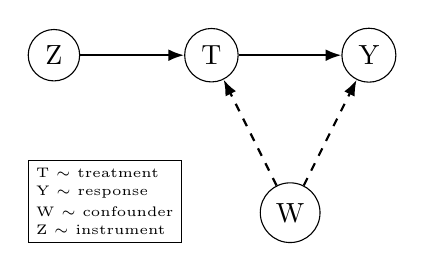
\begin{tikzpicture}[auto, node distance=2cm]

		\tikzstyle{edge} = [->, thick, -{Latex[length=2mm]}]
		\tikzstyle{edge_dashed} = [->, thick, -{Latex[length=2mm]}, dashed]
		\tikzstyle{vertex} = [circle, draw=black]

		\node[vertex](Z) at (0,0){Z};
		\node[vertex](T) [right of=Z]{T};
		\node[vertex](Y) [right of=T]{Y};
		\node[vertex](W) at(3, -2){W};

		\draw[edge] (Z) -- (T);
		\draw[edge] (T) -- (Y);
		\draw[edge_dashed] (W) -- (T);
		\draw[edge_dashed] (W) -- (Y);


		\matrix[draw, inner sep=0.5mm, above right] at  (current bounding box.south west)
		{
  		\node {\tiny T $\sim$ treatment}; \\
  		\node {\tiny Y $\sim$ response}; \\
  		\node {\tiny W $\sim$ confounder}; \\
  		\node {\tiny Z $\sim$ instrument}; \\
		};


  \end{tikzpicture}

\end{document}
